\newpage
\def\thoigian{90}%--Thời gian
\de{Đề số 3}{Chương II. Bất phương trình và hệ bất phương trình bậc nhất hai ẩn}
%\everymath{\color{blue}}
\begin{center}
	\textbf{PHẦN 1 - Câu trắc nghiệm nhiều phương án lựa chọn.}
\end{center}
\setcounter{ex}{0}
%============Câu 1=======================
\Opensolutionfile{ans}[ans-0D2-OTC-Deso3-ABCD]
\begin{ex}
	Trong các liên hệ giữa $x$ và $y$ cho sau đây, đâu là một bất phương trình bậc nhất hai ẩn? 
	\choice
	{$2x+y=1$}
	{$2x-y^{2}>0$}
	{\True $\sqrt{2}y-2x \le 1$}
	{$0x+0y \ge 5$}
	\loigiai{
		Bất phương trình $\sqrt{2}y-2x \le 1$ là một bất phương trình bậc nhất hai ẩn. 
	}
\end{ex}
\begin{ex}
	Cặp số nào sau đây là một nghiệm của hệ bất phương trình bậc nhất hai ẩn $\heva{&2x-3y < 2 \\ &x+y \ge 3}$?  
	\choice
	{$(0;-1)$}
	{\True $(2;1)$}
	{$(3;-1)$}
	{$(3;0)$}
	\loigiai{
		Thay $x=2$ và $y=1$ ta có $\heva{&2 \cdot 2-3 \cdot 1 < 2 \quad (\text{đúng}) \\ &2+1 \ge 3 \quad (\text{đúng}).}$ \\
		Vậy $(2;1)$ là một nghiệm của hệ bất phương trình đã cho. 
	}
\end{ex}
\begin{ex}
	Miền nghiệm của bất phương trình $x \ge 0$ được biểu diễn trên mặt phẳng tọa độ $Oxy$ là 
	\choice
	{Nửa mặt phẳng nằm phía dưới trục hoành (bao gồm cả trục hoành)}
	{Nửa mặt phẳng nằm phía trên trục hoành}
	{Nửa mặt phẳng nằm bên phải trục tung}
	{\True Nửa mặt phẳng nằm bên phải trục tung (bao gồm cả trục tung)}
	\loigiai{
		\immini{
			Miền nghiệm của bất phương trình $x \ge 0$ là nửa mặt phẳng nằm bên phải trục tung (bao gồm cả trục tung). 
		}
		{
			\begin{tikzpicture}[scale=0.7, >=stealth, line join=round, line cap=round, font=\footnotesize]
				\def\xmin{-2} 
				\def\xmax{2}
				\def\ymin{-2} 
				\def\ymax{2} 
				\draw [->] (\xmin,0)--(\xmax,0) node [below, xshift=-3pt] {$x$};
				\draw [->] (0,\ymin)--(0,\ymax) node [left, yshift=-4pt] {$y$};
				\draw (0,\ymax) node [right, yshift=-4pt] {$x=0$};
				\draw [fill=black] (0,0) circle (1pt) node [below left] {$O$};
				\clip (\xmin,\ymin) rectangle (\xmax,\ymax);
				%
				\fill [pattern=north east lines] 
				plot [domain=\ymin:\ymax+1] ({0}, {\x})--plot [domain=\ymax+1:\ymin] (\xmin-1, {\x});
			\end{tikzpicture}
		}
	}
\end{ex}
\begin{ex}
	Miền nghiệm của bất phương trình $x+3y<-1$ được biểu diễn trên mặt phẳng tọa độ $Oxy$ là 
	\choice
	{Nửa mặt phẳng có bờ là đường thẳng $x+3y=-1$, không chứa điểm $O(0;0)$ (kể cả bờ)}
	{Nửa mặt phẳng có bờ là đường thẳng $x+3y=-1$, có chứa điểm $O(0;0)$ (kể cả bờ)}
	{Nửa mặt phẳng có bờ là đường thẳng $x+3y=-1$, có chứa điểm $O(0;0)$}
	{\True Nửa mặt phẳng có bờ là đường thẳng $x+3y=-1$, không chứa điểm $O(0;0)$}
	\loigiai{
		Thay $x=0$ và $y=0$ ta có 
		$$0+3 \cdot 0<-1 \quad \text{(sai)}.$$ 
		Vậy miền nghiệm của bất phương trình $x+3y<-1$ là nửa mặt phẳng có bờ là đường thẳng $x+3y=-1$, không chứa điểm $O(0;0)$.
	}
\end{ex}
\begin{ex}
	\immini{
		Phần hình phẳng không bị gạch ở hình bên biểu diễn miền nghiệm của bất phương trình nào sau đây?
		\choice[1]
		{\True $x+2y<4$}
		{$x+2y \le 4$}
		{$x+2y>4$}
		{$x+2y \ge 4$}
	}
	{
		\begin{tikzpicture}[scale=0.7, >=stealth, line join=round, line cap=round, font=\footnotesize]
			% Định nghĩa khung
			\def\xmin{-1}
			\def\xmax{5}
			\def\ymin{-1}
			\def\ymax{3}
			\def\a{1} 
			\def\b{2} 
			\def\c{4} 
			\pgfmathsetmacro\m{-\a/\b}
			\pgfmathsetmacro\n{\c/\b}
			% Định nghĩa hàm số
			\def\f{\m*(\x)+\n}
			% Vẽ hệ trục
			\draw [->] (\xmin,0)--(\xmax,0) node [below, xshift=-3pt] {$x$};
			\draw [->] (0,\ymin)--(0,\ymax) node [left, yshift=-4pt] {$y$};
			\draw [smooth, samples=100, dashed, thick] plot [domain=\xmin:\xmax] (\x, {\f}) node [below] {$d \colon x+2y=4$};
			\draw [fill=black] (0,0) circle (1pt) node [below left] {$O$}
			(0,2) circle (1pt) node [below left] {$2$}
			(4,0) circle (1pt) node [below] {$4$};
			% Cắt hình
			\clip (\xmin,\ymin) rectangle (\xmax,\ymax);
			\fill [pattern=north east lines] plot [domain=\xmin:\xmax+1] (\x, {\f})--plot [domain=\xmax+1:\xmin] (\x, {\ymax+1});
		\end{tikzpicture}
	}
	\loigiai{
		Xét điểm $O(0;0)$ (không thuộc $d$) và thuộc miền nghiệm của bất phương trình. \\
		Thay $x=0$ và $y=0$ ta có 
		$$0+2 \cdot 0<4.$$
		Vậy phần hình phẳng không bị gạch biểu diễn miền nghiệm của bất phương trình $x+2y<4$. 
	}
\end{ex}
\begin{ex}
	\immini{
		Phần hình phẳng không bị gạch ở hình bên biểu diễn miền nghiệm của bất phương trình nào sau đây?
		\motcot
		{$y \le 1$}
		{$y>1$}
		{\True $y \ge 1$}
		{$x \le 1$}
	}
	{
		\begin{tikzpicture}[scale=0.7, >=stealth, line join=round, line cap=round, font=\footnotesize]
			% Định nghĩa khung
			\def\xmin{-2}
			\def\xmax{2}
			\def\ymin{-1}
			\def\ymax{3}
			%
			\draw [fill=black] (0,0) circle (1pt) node [below left] {$O$}
			(0,1) circle (1pt) node [above left] {$1$};
			\draw [thick] (\xmin,1)--(\xmax,1);
			% Cắt hình
			\clip (\xmin,\ymin) rectangle (\xmax,\ymax);
			\fill [pattern=north east lines]
			plot [domain=\xmin:\xmax+1] (\x, {1})--plot [domain=\xmax+1:\xmin] (\x, {\ymin-1});
			\draw [->] (\xmin,0)--(\xmax,0) node [below=2pt, xshift=-3pt, fill=white, inner sep=1pt] {$x$};
			\draw [->] (0,\ymin)--(0,\ymax) node [left=2pt, yshift=-3pt, fill=white, inner sep=1pt] {$y$};
		\end{tikzpicture}
	}
	\loigiai{
		Phần hình phẳng không bị gạch là nửa mặt phẳng có bờ là đường thẳng $y=1$ và không chứa điểm $O(0;0)$ nên là miền nghiệm của bất phương trình $y \ge 1$. 
	}
\end{ex}
%
\begin{ex}
	Bạn Nam mua $x$ quyển vở và $y$ chiếc bút. Mỗi quyển vở giá $12$ nghìn đồng, mỗi chiếc bút giá $8$ nghìn đồng ($x$, $y \in \mathbb{N}^*$). Nếu Nam có $10$ nghìn đồng và số quyển vở Nam mua nhiều hơn số chiếc bút thì $x$ và $y$ phải thỏa mãn hệ bất phương trình nào sau đây? 
	\choice 
	{$\heva{&x-y \le 0 \\ &3x+2y \le 25}$}
	{$\heva{&x-y \ge 0 \\ &3x+2y \le 50}$}
	{\True $\heva{&x-y>0 \\ &3x+2y \le 25}$}
	{$\heva{&x+y>0 \\ &3x+2y \ge 25}$}
	\loigiai{
		Vì số quyển vở nhiều hơn số chiếc bút nên ta có 
		$$x>y \quad \text{hay} \quad x-y>0.$$
		Số tiền Nam sử dụng để mua $x$ quyển vở và $y$ chiếc bút là $12x+8y$ (nghìn đồng). \\
		Vì Nam có $100$ (nghìn đồng) nên \\
		$$12x+8y \le 100 \quad \text{hay} \quad 3x+y \le 25.$$
		Vậy $x$, $y$ thỏa mãn hệ bất phương trình $\heva{&x-y>0 \\ &3x+2y \le 25.}$
	}
\end{ex}
\begin{ex}
	\immini[thm]{
		Phần hình phẳng {\bf không} bị gạch ở hình bên biểu diễn miền nghiệm của bất phương trình nào sau đây? 
		\choice[1]
		{$x+y \le 3$}
		{\True $x+y \ge 3$}
		{$2x-y \le 3$}
		{$2x-y \ge 3$}
	}
	{
		\begin{tikzpicture}[scale=0.6, >=stealth, line join=round, line cap=round, font=\footnotesize]
			% Định nghĩa khung
			\def\xmin{-1}
			\def\xmax{4}
			\def\ymin{-1}
			\def\ymax{4}
			\def\a{1} 
			\def\b{1} 
			\def\c{3} 
			\pgfmathsetmacro\m{-\a/\b}
			\pgfmathsetmacro\n{\c/\b}
			\def\f{\m*(\x)+\n}
			% 
			\draw [fill=black] (0,0) circle (0.05) node [below left] {$O$}
			(0,3) circle (1pt) node [right] {$3$} 
			(3,0) circle (1pt) node [above] {$3$};
			% Cắt hình
			\clip (\xmin,\ymin) rectangle (\xmax,\ymax);
			\fill [pattern=north east lines, draw, thick]
			plot [domain=\xmin:\xmax+1] (\x, {\f})--plot [domain=\xmax+1:\xmin] (\x, {\ymin-1});
			%
			\draw [->] (\xmin,0)--(\xmax,0) node [below=2pt, xshift=-3pt, fill=white, inner sep=1pt] {$x$};
			\draw [->] (0,\ymin)--(0,\ymax) node [left=2pt, yshift=-3pt, fill=white, inner sep=1pt] {$y$};
		\end{tikzpicture}
	}
	\loigiai{
		Gọi $d$ là đường thẳng đi qua hai điểm $(0;3)$ và $(3;0)$. \\
		Khi đó $d$ có phương trình $x+y=3$. \\
		Xét điểm $O(0;0)$ không thuộc miền nghiệm. \\
		Thay $x=0$ và $y=0$ ta có $0+0<3$. \\
		Vậy phần hình phẳng không bị gạch là miền nghiệm của bất phương trình $x+y \ge 3$. 
	}
\end{ex}
\begin{ex}
	\immini{
		Tam giác $OAB$ ở hình bên biểu diễn miền nghiệm của hệ bất phương trình bậc nhất hai ẩn nào sau đây? 
		\choice[2]
		{$\heva{&x \ge 0 \\ &x-y \le 0 \\ &2x+y \le 3}$}
		{\True $\heva{&x \ge 0 \\ &x-y \ge 0 \\ &2x+y \le 3}$}
		{$\heva{&x \le 0 \\ &x-y \ge 0 \\ &2x+y \le 3}$}
		{$\heva{&x \ge 0 \\ &x-y \ge 0 \\ &2x+y \ge 3}$}
	}
	{
		\begin{tikzpicture}[scale=0.6, >=stealth, line join=round, line cap=round, font=\footnotesize]
			% Định nghĩa khung
			\def\xmin{-1}; 
			\def\xmax{4}; 
			\def\ymin{-1}; 
			\def\ymax{4}; 
			% Cắt hình
			\clip (\xmin,\ymin) rectangle (\xmax,\ymax);
			%
			\fill [pattern=vertical lines]
			plot [domain=\xmin:\xmax+1] (\x, {0})--plot [domain=\xmax+1:\xmin] (\x, {\ymin-1});
			%
			\fill [pattern=north west lines, draw, thick]
			plot [domain=\xmin:\xmax] (\x, {\x})--plot [domain=\xmax+1:\xmin] (\x, {\ymax+1});
			%
			\fill [pattern=north east lines, draw, thick]
			plot [domain=\xmin:\xmax] (\x, {-2*(\x)+3})--plot [domain=\xmax+1:\xmin] (\x, {\ymax+1});
			%
			\draw [dashed] (1,0)--(1,1)--(0,1);
			% Vẽ hệ trục
			\draw [->] (\xmin,0)--(\xmax,0) node [below=2pt, xshift=-3pt, fill=white, inner sep=1pt] {$x$};
			\draw [->] (0,\ymin)--(0,\ymax) node [left=2pt, yshift=-3pt, fill=white, inner sep=1pt] {$y$};
			\draw [fill=black] (0,0) circle (1pt) ++(-135:.5) node [fill=white, inner sep=1pt] {$O$}
			(1.5,0) circle (1pt) node [below=2pt, fill=white, inner sep=1pt] {$\frac{3}{2}$}
			(1,0) circle (1pt) node [below=2pt, fill=white, inner sep=1pt] {$1$} 
			(0,1) circle (1pt) ++(180:.4) node [fill=white, inner sep=1pt] {$1$}
			(0,3) circle (1pt) ++(180:.4) node [fill=white, inner sep=1pt] {$3$}
			(1,1) circle (1pt) ++(90:.4) node [fill=white, inner sep=1pt] {$A$}
			(1.5,0) circle (1pt) ++(45:.4) node [fill=white, inner sep=1pt] {$B$}; 
		\end{tikzpicture}
	}
	\loigiai{
		\immini{
			Chọn điểm $M\left(1;\dfrac{1}{2}\right)$ thuộc miền trong của tam giác $OAB$. \\
			Thay $x=1$ và $y=\dfrac{1}{2}$ ta có 
			$$\heva{&1 \ge 0 \\ &1-\dfrac{1}{2} \ge 0 \\ &2 \cdot 1+\dfrac{1}{2} \le 3}.$$
			Vậy tam giác $OAB$ là miền nghiệm của hệ bất phương trình $\heva{&x \ge 0 \\ &x-y \ge 0 \\ &2x+y \le 3}$. 
		}{
			\begin{tikzpicture}[scale=0.6, >=stealth, line join=round, line cap=round, font=\footnotesize]
				% Định nghĩa khung
				\def\xmin{-1}; 
				\def\xmax{4}; 
				\def\ymin{-1}; 
				\def\ymax{4}; 
				% Cắt hình
				\clip (\xmin,\ymin) rectangle (\xmax,\ymax);
				%
				\fill [pattern=vertical lines]
				plot [domain=\xmin:\xmax+1] (\x, {0})--plot [domain=\xmax+1:\xmin] (\x, {\ymin-1});
				%
				\fill [pattern=north west lines, draw, thick]
				plot [domain=\xmin:\xmax] (\x, {\x})--plot [domain=\xmax+1:\xmin] (\x, {\ymax+1});
				%
				\fill [pattern=north east lines, draw, thick]
				plot [domain=\xmin:\xmax] (\x, {-2*(\x)+3})--plot [domain=\xmax+1:\xmin] (\x, {\ymax+1});
				%
				\draw [dashed] (1,0)--(1,1)--(0,1) (0,.5)--(1,.5);
				% Vẽ hệ trục
				\draw [->] (\xmin,0)--(\xmax,0) node [below=2pt, xshift=-3pt, fill=white, inner sep=1pt] {$x$};
				\draw [->] (0,\ymin)--(0,\ymax) node [left=2pt, yshift=-3pt, fill=white, inner sep=1pt] {$y$};
				\draw [fill=black] (0,0) circle (1pt) ++(-135:.5) node [fill=white, inner sep=1pt] {$O$}
				(1.5,0) circle (1pt) node [below=2pt, fill=white, inner sep=1pt] {$\frac{3}{2}$}
				(1,0) circle (1pt) node [below=2pt, fill=white, inner sep=1pt] {$1$} 
				(0,1) circle (1pt) ++(180:.4) node [fill=white, inner sep=1pt] {$1$}
				(0,.5) circle (1pt) ++(180:.4) node [fill=white, inner sep=1pt] {$0{,}5$}
				(0,3) circle (1pt) ++(180:.4) node [fill=white, inner sep=1pt] {$3$}
				(1,1) circle (1pt) ++(90:.4) node [fill=white, inner sep=1pt] {$A$}
				(1.5,0) circle (1pt) ++(45:.4) node [fill=white, inner sep=1pt] {$B$}
				(1,.5) circle (1pt) ++(0:.4) node [fill=white, inner sep=1pt] {$M$}; 
			\end{tikzpicture}
		}
	}
\end{ex}
\begin{ex}
	\immini[thm]{
		Phần hình phẳng không bị gạch trên mặt phẳng tọa độ ở hình bên biểu diễn miền nghiệm của hệ bất phương trình bậc nhất hai ẩn nào sau đây? 
		\haicot
		{$\heva{&y \ge 0 \\ &x \ge 0 \\ &x+y \le 2}$}
		{\True $\heva{&x \ge 0 \\ &y \ge 0 \\ &x+y \ge 2}$}
		{$\heva{&x \ge 0 \\ &y \le 0 \\ &x+y \ge 2}$}
		{$\heva{&x \le 0 \\ &y \ge 0 \\ &x+y \ge 2}$}
	}
	{
		\begin{tikzpicture}[scale=0.7, >=stealth, line join=round, line cap=round, font=\footnotesize]
			% Định nghĩa khung
			\def\xmin{-1}
			\def\xmax{3}
			\def\ymin{-1}
			\def\ymax{3} 
			% 
			\clip (\xmin,\ymin) rectangle (\xmax,\ymax);
			%
			\fill [pattern=north west lines]
			plot [domain=\ymin:\ymax+1] ({0}, {\x})--plot [domain=\ymax+1:\ymin] ({\xmin-1},\x);
			%
			\fill [pattern=north east lines]
			plot [domain=\xmin:\xmax+1] (\x, {0})--plot [domain=\xmax+1:\xmin] (\x, {\ymin-1});
			%
			\fill [pattern=vertical lines, draw, thick]
			plot [domain=\xmin:\xmax] (\x, {-(\x)+2})--plot [domain=\xmax+1:\xmin] (\x, {\ymin-1});
			%
			\draw [->] (\xmin,0)--(\xmax,0) node [below=2pt, xshift=-3pt, fill=white, inner sep=1pt] {$x$};
			\draw [->] (0,\ymin)--(0,\ymax) node [left=2pt, yshift=-3pt, fill=white, inner sep=1pt] {$y$};
			\draw [fill=black] (0,0) circle (1pt) node [below left] {$O$}
			(2,0) circle (1pt) node [above] {$2$}
			(0,2) circle (1pt) node [right] {$2$}
			;
		\end{tikzpicture}
	}
	\loigiai{
		\immini{
			Lấy điểm $M(2;2)$ thuộc miền nghiệm. \\
			Thay $x=2$ và $y=2$ ta có 
			$$\heva{&2 \ge 0 \\ &2 \ge 0 \\ &2+2 \ge 2}.$$
			Vậy phần hình phẳng không bị gạch ở hình bên biểu diễn miền nghiệm của bất phương trình $\heva{&x \ge 0 \\ &y \ge 0 \\ &x+y \ge 2.}$
		}{
			\begin{tikzpicture}[scale=0.7, >=stealth, line join=round, line cap=round, font=\footnotesize]
				% Định nghĩa khung
				\def\xmin{-1}
				\def\xmax{3}
				\def\ymin{-1}
				\def\ymax{3} 
				% Cắt hình
				\clip (\xmin,\ymin) rectangle (\xmax,\ymax);
				%
				\fill [pattern=north west lines]
				plot [domain=\ymin:\ymax+1] ({0}, {\x})--plot [domain=\ymax+1:\ymin] ({\xmin-1},\x);
				%
				\fill [pattern=north east lines]
				plot [domain=\xmin:\xmax+1] (\x, {0})--plot [domain=\xmax+1:\xmin] (\x, {\ymin-1});
				%
				\fill [pattern=vertical lines, draw, thick]
				plot [domain=\xmin:\xmax] (\x, {-(\x)+2})--plot [domain=\xmax+1:\xmin] (\x, {\ymin-1});
				%
				\draw [->] (\xmin,0)--(\xmax,0) node [below=2pt, xshift=-3pt, fill=white, inner sep=1pt] {$x$};
				\draw [->] (0,\ymin)--(0,\ymax) node [left=2pt, yshift=-3pt, fill=white, inner sep=1pt] {$y$};
				\draw [fill=black] (0,0) circle (1pt) node [below left] {$O$}
				(2,0) circle (1pt) node [above] {$2$}
				(0,2) circle (1pt) node [right] {$2$}
				;
			\end{tikzpicture}
		}
	}
\end{ex}
\begin{ex}
	Một quán ăn trong khu du lịch niêm yết giá cho mỗi suất ăn như sau 
	\begin{itemize}
		\item Suất cho người lớn: $45\;000$ đồng. 
		\item Suất ăn cho trẻ em: $30\,000$ đồng. 
	\end{itemize}
	Theo như chủ quán tính toán, để không phải bù lỗ thì doanh thu một ngày của quán phải không ít hơn $5$ triệu đồng. Gọi $x$ là số suất ăn cho người lớn và $y$ là số suất ăn cho trẻ em mà quán được trong một ngày $(x, \; y \in \mathbb{N})$. Để không phải bù lỗ thì $x$ và $y$ phải thỏa mãn hệ thức nào sau đây?
	\choice 
	{$9x+6y \le 5\,000$}
	{$9x+6y \ge 5\,000$}
	{\True $9x+6y \ge 1\,000$} 
	{$9x+6y > 1\,000$}
	\loigiai{
		Doanh thu một ngày của quán ăn là 
		$$45\,000x+30\,000y \; (\text{đồng}).$$
		Để không phải bù lỗ thì doanh thu một ngày của quán phải không ít hơn $5$ triệu đồng nên ta có 
		$$45\,000x+30\,000y \ge 5\,000\,000 \text{ hay } 9x+6y \ge 1\,000.$$
	}
\end{ex}
\begin{ex}
	\immini{
		Trong mặt phẳng tọa độ $Oxy$, cho tứ giác $ABCD$ như hình vẽ bên. Gọi $(x;y)$ là điểm thuộc miền tứ giác $ABCD$ (điểm thuộc miền trong hoặc nằm trên các cạnh của tứ giác). Tìm giá trị nhỏ nhất của biểu thức $T(x;y)=2\,025x-2\,026y$?
		\choice[1]
		{$-10\,124$}
		{$-2\,026$}
		{$-1$}
		{\True $-4\,054$}
	}
	{
		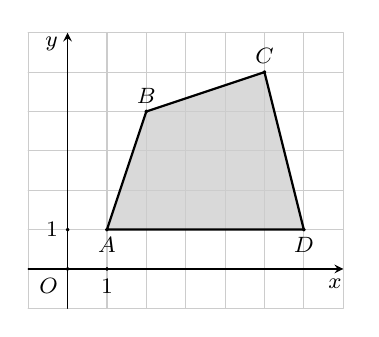
\begin{tikzpicture}[scale=0.5, >=stealth, line join=round, line cap=round, font=\footnotesize]
			\def\xmin{-1} 
			\def\xmax{7}
			\def\ymin{-1} 
			\def\ymax{6} 
			\fill [gray!30] (1,1)--(2,4)--(5,5)--(6,1)--cycle;
			\draw [gray!40] (\xmin,\ymin) grid (\xmax,\ymax);
			\draw [->] (\xmin,0)--(\xmax,0) node [below, xshift=-3pt] {$x$};
			\draw [->] (0,\ymin)--(0,\ymax) node [left, yshift=-4pt] {$y$};
			\draw [fill=black] (0,0) circle (1pt) node [below left] {$O$}
			(1,1) circle (1pt) ++(-90:.4) node {$A$}
			(2,4) circle (1pt) ++(90:.4) node {$B$}
			(5,5) circle (1pt) ++(90:.4) node {$C$}
			(6,1) circle (1pt) ++(-90:.4) node {$D$}
			(1,0) circle (1pt) node [below] {$1$}
			(0,1) circle (1pt) node [left] {$1$};
			\draw [thick] (1,1)--(2,4)--(5,5)--(6,1)--cycle;
		\end{tikzpicture}
	}
	\loigiai{
		Giá trị nhỏ nhất của biểu thức $T(x;y)=2\,025x-2\,026y$ đạt được tại đỉnh của tứ giác $ABCD$. \\
		Tại các đỉnh $A$, $B$, $C$, $D$ thì giá trị của biểu thức $T(x;y)$ lần lượt là 
		\begin{eqnarray*}
			&&T(1;1) = 2\,025 \cdot 1-2\,026 \cdot 1 = -1. \\
			&&T(2;4) = 2\,025 \cdot 2-2\,026 \cdot 4 = -4\,054. \\
			&&T(5;5) = 2\,025 \cdot 5-2\,026 \cdot 5 = -5. \\
			&&T(6;1) = 2\,025 \cdot 6-2\,026 \cdot 1 = 10\,124.
		\end{eqnarray*}
		Vậy $T(x;y)$ đạt giá trị nhỏ nhất bằng $-4\,054$. 
	}
\end{ex}
\Closesolutionfile{ans}

\begin{center}
	\textbf{PHẦN 2 - Câu trắc nghiệm đúng sai. Trong mỗi ý a,b,c,d ở mỗi câu, thí sinh chọn đúng hoặc sai}
\end{center}

\setcounter{ex}{0}
\Opensolutionfile{ans}[ans-0D2-OTC-Deso3-DS]
\begin{ex}
	Cho bất phương trình bậc nhất hai ẩn $2\,025x-2\,026y<0$ có miền nghiệm được biểu diễn trên mặt phẳng tọa độ $Oxy$. 
	\choiceTF
	{\True Bất phương trình đã cho có vô số nghiệm}
	{\True Cặp số $\left(\sqrt{2};\sqrt{3}\right)$ là một nghiệm của bất phương trình đã cho}
	{Điểm $O(0;0)$ thuộc miền nghiệm của bất phương trình đã cho}
	{Miền nghiệm của bất phương trình đã cho là nửa mặt phẳng có bờ là đường thẳng $2\,025x-2\,026y=0$, không chứa điểm $M(0;1)$}
	\loigiai{
		\begin{itemchoice}
			\itemch Bất phương trình bậc nhất hai ẩn có vô số nghiệm. 
			\itemch Thay $x=\sqrt{2}$ và $y=\sqrt{3}$ ta có 
			$$2\,025 \cdot \sqrt{2}-2\,025 \cdot \sqrt{3}<0 \quad \text{(đúng)}.$$
			Vậy cặp số $\left(\sqrt{2};\sqrt{3}\right)$ là một nghiệm của bất phương trình đã cho. 
			\itemch Thay $x=0$ và $y=0$ ta có 
			$$2\,025 \cdot 0-2\,026 \cdot 0<0 \quad \text{(sai)}.$$
			Vậy điểm $O(0;0)$ không thuộc miền nghiệm của bất phương trình đã cho. 
			\itemch Thay $x=0$ và $y=1$ ta có 
			$$2\,025 \cdot 0-2\,026 \cdot 1<0 \quad \text{(đúng)}.$$
			Vậy miền nghiệm của bất phương trình đã cho là nửa mặt phẳng có bờ là đường thẳng $2\,025x-2\,026y=0$, chứa điểm $M(0;1)$
		\end{itemchoice}
	}
\end{ex}
\begin{ex}
	Một cửa hàng kinh doanh hai loại sản phẩm: sản phẩm loại (I) và sản phẩm loại (II). Mỗi sản phẩm loại (I) tốn chi phí sản xuất là $100$ nghìn đồng và thu lợi nhuận $40$ nghìn đồng. Mỗi sản phẩm loại (II) tốn chi phí sản suất là $80$ nghìn đồng và thu lợi nhuận $30$ nghìn đồng (giả sử tất cả sản phẩm sản suất ra đều được bán hết). Gọi $x$ và $y$ lần lượt là số lượng sản phẩm loại (I) và loại (II) bán được trong một tháng $(x, \; y \in \mathbb{N})$. Biết rằng cửa hàng kinh doanh nhỏ nên trong một tháng chỉ có thể bỏ ra số tiền vốn tối đa $8$ triệu đồng để sản suất sản phẩm. 
	\choiceTF
	{\True Chi phí sản suất hai loại sản phẩm trong một tháng là $100x+80y$ (nghìn đồng)}
	{\True Lợi nhuận cửa hàng thu được trong một tháng là $40x+30y$ (nghìn đồng)} 
	{Các số $x$ và $y$ thỏa mãn hệ bất phương trình $\heva{&x \ge 0, \; y \ge 0 \\ &5x+4y \le 200}$} 
	{Lợi nhuận của cửa hàng trong một tháng không vượt quá $3$ triệu đồng}
	\loigiai{
		\immini{
			\begin{itemchoice}
				\itemch Chi phí sản suất $x$ sản phẩm loại (I) và $y$ sản phẩm loại (II) là 
				$$100x+80y \quad \text{(nghìn đồng)}.$$
				\itemch Lợi nhuận thu được khi bán $x$ sản phẩm loại (I) và $y$ sản phẩm loại (II) là 
				$$40x+30y \quad \text{(nghìn đồng)}.$$
				\itemch Theo đề $x, \; y \in \mathbb{N}$ nên $x \ge 0$, $y \ge 0$. \\
				Vì chi phí sản suất một tháng tối đa $8$ triệu đồng nên 
				$$100x+80y \le 8\,000 \quad \text{hay} \quad 5x+4y \le 400.$$
				Vậy các số $x$, $y$ thỏa mãn hệ bất phương trình $\heva{&x \ge 0, \; y \ge 0 \\ &5x+4y \le 400} \quad (*)$.
				\itemch Miền nghiệm của hệ bất phương trình $(*)$ là tam giác $OAB$ với $O(0;0)$, $A(0;100)$ và $B(80;0)$. \\
				Lợi nhuận thu được một tháng là $F(x;y)=40x+30y$ (nghìn đồng). \\
				Biểu thức $F(x;y)$ đạt giá trị lớn nhất tại đỉnh của tam giác $OAB$. \\
				Ta có 
				\begin{eqnarray*}
					&&F(0;0)=40 \cdot 0+30 \cdot 0=0. \\
					&&F(0;100)=40 \cdot 0+30 \cdot 100=3\,000. \\
					&&F(80;0)=40 \cdot 80+30 \cdot 0=3\,200.
				\end{eqnarray*}
				Do đó $F(x;y)$ đạt giá trị lớn nhất bằng $3\,200$. \\
				Vậy lợi nhuận của cửa hàng trong một tháng không vượt quá $3{,}2$ triệu đồng. 
			\end{itemchoice}
		}
		{
			\begin{tikzpicture}[scale=.04, >=stealth, line join=round, line cap=round, font=\footnotesize]
				\def\xmin{-20} 
				\def\xmax{100}
				\def\ymin{-20} 
				\def\ymax{120} 
				%
				\clip (\xmin,\ymin) rectangle (\xmax,\ymax);
				\fill [pattern=horizontal lines]
				plot [domain=\ymin:\ymax+1] ({0}, {\x})--plot [domain=\ymax+1:\ymin] ({\xmin-1},\x);
				%
				\fill [pattern=vertical lines, thick]
				plot [domain=\xmin:\xmax+1] (\x, {0})--plot [domain=\xmax+1:\xmin] (\x, {\ymin-1});
				%
				\def\f{(-5/4)*(\x)+100}
				\fill [pattern=north east lines, draw, thick]
				plot [domain=\xmin:\xmax] (\x, {\f})--plot [domain=\xmax+1:\xmin] (\x, {\ymax+1});
				%
				\draw [->] (\xmin,0)--(\xmax,0) ++(-90:8) node [xshift=-3pt, fill=white, inner sep=1pt] {$x$};
				\draw [->] (0,\ymin)--(0,\ymax) ++(180:8) node [yshift=-4pt, fill=white, inner sep=1pt] {$y$};
				\draw [fill=black] (0,0) circle (1pt) ++(-135:8) node [fill=white, inner sep=.5pt] {$O$}
				(80,0) circle (1pt) ++(-110:8) node [fill=white, inner sep=1pt] {$80$}
				(80,0) ++(90:8) node [fill=white, inner sep=.5pt] {$B$}
				(0,100) circle (1pt) ++(180:10) node [fill=white, inner sep=1pt] {$100$}
				(0,100) ++(0:8) node [fill=white, inner sep=.5pt] {$A$}
				;
			\end{tikzpicture}
		}
	}
\end{ex}

\Closesolutionfile{ans}

\begin{center}
	\textbf{PHẦN 3 - Câu trắc nghiệm trả lời ngắn}
\end{center}
\setcounter{ex}{0}

\Opensolutionfile{ans}[ans-0D2-OTC-Deso3-KQ]
\begin{ex}
	Một nhân viên siêu thị điện máy được trả khoản tiền hoa hồng cho mỗi tivi bán được là $100$ nghìn đồng và mỗi điện thoại bán được là $80$ nghìn đồng. Gọi $x$ và $y$ lần lượt là số tivi và số điện thoại mà một nhân viên bán được trong một tháng $(x, \; y \in \mathbb{N})$. Nếu trong một tháng nhân viên nhận được số tiền hoa hồng không ít hơn $2$ triệu đồng thì $x$ và $y$ thỏa mãn bất phương trình $ax+by \ge 100$. Tính giá trị $a^2+b^2$. 
	\shortans[oly]{$41$}
	\loigiai{
		Số tiền hoa hồng nhân viên nhận được trong một tháng là $100x+80y$ (nghìn đồng). \\
		Theo đề ta có bất phương trình 
		$$100x+80y \ge 2\,000 \quad \text{hay} \quad 5x+4y \ge 100.$$ 
		Suy ra $a=5$ và $b=4$. \\
		Vậy $a^2+b^2=5^2+4^2=41$. 
	}
\end{ex}
\begin{ex}
	Trong mặt phẳng tọa độ $Oxy$, miền nghiệm của hệ bất phương trình $\heva{&y \ge 0 \\ &x-y \ge 0 \\ &x+y \le 4}$ có chứa bao nhiêu điểm có tọa độ là số nguyên?
	\shortans[oly]{$8$}
	\loigiai{
		\immini{
			Xét các đường thẳng $y=0$ (trục hoành), $d \colon x-y=0$ và $d' \colon x+y=4$. \\
			Chọn điểm $M(2;1)$ không thuộc các đường thẳng trên.
			\begin{itemize}
				\item Với bất phương trình $y \ge 0$ \\
				Có $1>0$ nên miền nghiệm của bất phương trình $y \ge 0$ là nửa mặt phẳng có bờ là đường thẳng $y=0$, có chứa điểm $M(2;1)$ (kể cả bờ). 
				\item Với bất phương trình $x-y \ge 0$ \\
				Có $2-1=1>0$ nên miền nghiệm của bất phương trình $x-y \ge 0$ là nửa mặt phẳng có bờ là đường thẳng $d$, có chứa điểm $M(2;1)$ (kể cả bờ). 
				\item Với bất phương trình $x+y \le 4$ \\
				Có $2+1=3<4$ nên miền nghiệm của bất phương trình $x+y \le 4$ là nửa mặt phẳng có bờ là đường thẳng $d'$, có chứa điểm $M(2;1)$ (kể cả bờ). 
			\end{itemize} 
			Gọi $A$ là giao điểm giữa $d$ và $d'$, $B$ là giao điểm của $d'$ và trục hoành. \\
			Suy ra $A(2;2)$ và $B(4;0)$. \\
			Miền nghiệm của hệ bất phương trình đã cho là tam giác $OAB$. \\
			Các điểm có tọa độ nguyên thuộc miền của tam giác $OAB$ là \\
			$(0;0)$, $(1;0)$, $(1;1)$, $(2;0)$, $(2;1)$, $(2;2)$, $(3;0)$, $(3;1)$, $(4;0)$. \\
			Vậy có $8$ điểm thỏa mãn yêu cầu đề bài. 
		}  
		{
			\begin{tikzpicture}[scale=0.7, >=stealth, line join=round, line cap=round, font=\footnotesize]
				\def\xmin{-1} 
				\def\xmax{5}
				\def\ymin{-1} 
				\def\ymax{5} 
				\clip (\xmin,\ymin) rectangle (\xmax,\ymax);
				\draw [gray!30] (\xmin,\ymin) grid (\xmax,\ymax);
				%
				\fill [pattern=vertical lines]
				plot [domain=\xmin:\xmax+1] (\x, {0})--plot [domain=\xmax+1:\xmin] (\x, {\ymin-1});
				%
				\fill [pattern=north west lines, draw, thick]
				plot [domain=\xmin:\xmax] (\x, {\x})--plot [domain=\xmax+1:\xmin] (\x, {\ymax+1})
				;
				%
				\fill [pattern=north east lines, draw, thick]
				plot [domain=\xmin:\xmax] (\x, {4-\x})--plot [domain=\xmax+1:\xmin] (\x, {\ymax+1});
				%
				\draw [->] (\xmin,0)--(\xmax,0) node [below=2pt, xshift=-3pt, fill=white, inner sep=1pt] {$x$};
				\draw [->] (0,\ymin)--(0,\ymax) node [left=2pt, yshift=-3pt, fill=white, inner sep=1pt] {$y$};
				\draw [dashed] (2,0)--(2,2)--(0,2);
				\draw [fill=black] (0,0) circle (1pt) ++(-135:.5) node [fill=white, inner sep=.5pt] {$O$}
				(4,0) circle (1pt) ++(-110:.4) node [fill=white, inner sep=1pt] {$4$}
				(4,0) ++(90:.5) node [fill=white, inner sep=.5pt] {$B$}
				(0,4) circle (1pt) ++(180:.4) node [fill=white, inner sep=1pt] {$4$}
				(2,2) ++(90:.5) node [fill=white, inner sep=.5pt] {$A$}
				(.8,3.2) node [above=2pt, rotate=-45, fill=white, inner sep=.5pt] {$d \colon x+y=4$}
				(3.5,3.5) node [above=2pt, rotate=45, fill=white, inner sep=.5pt] {$d' \colon x-y=0$}
				(2,0) circle (1pt) ++(-90:.4) node [fill=white, inner sep=1pt] {$2$}
				(0,2) circle (1pt) ++(180:.4) node [fill=white, inner sep=1pt] {$2$}
				;
			\end{tikzpicture}
		}
	}
\end{ex}
\begin{ex}
	Tìm giá trị lớn nhất của biểu thức $F(x;y)=5x+3y$ biết $(x;y)$ thuộc miền nghiệm của hệ bất phương trình $\heva{&x \ge -1 \\ &x+y \le 2 \\ &y \ge 0}$. 
	\shortans[oly]{$15$}
	\loigiai{
		\immini{
			Xét các đường thẳng $d_1 \colon x=-1$, $d_2 \colon x+y=2$ và $y=0$ (trục hoành). \\
			Chọn điểm $M(0;1)$ không thuộc các đường thẳng trên.
			\begin{itemize}
				\item Với bất phương trình $x \ge -1$ \\
				Có $0>-1$ nên miền nghiệm của bất phương trình $x \ge -1$ là nửa mặt phẳng có bờ là đường thẳng $d_1$, có chứa điểm $M(0;1)$ (kể cả bờ). 
				\item Với bất phương trình $x+y \le 2$ \\
				Có $0+1=1<2$ nên miền nghiệm của bất phương trình $x+y \le 2$ là nửa mặt phẳng có bờ là đường thẳng $d_2$, có chứa điểm $M(0;1)$ (kể cả bờ). 
				\item Với bất phương trình $y \ge 0$ \\
				Có $1>0$ nên miền nghiệm của bất phương trình $y \ge 0$ là nửa mặt phẳng có bờ là trục hoành, có chứa điểm $M(0;1)$ (kể cả bờ). 
			\end{itemize} 
			Gọi $A$ là giao điểm của $d_1$ và trục hoành, $B$ là giao điểm của $d_2$ và trục hoành, $C$ là giao điểm của $d_1$ và $d_2$. \\
			Suy ra $A(-1;0)$, $B(-1;3)$ và $C(3;0)$. \\
			Miền nghiệm của hệ bất phương trình đã cho là tam giác $ABC$. \\
			Biểu thức $T(x;y)=5x+3y$ đạt giá trị nhỏ nhất tại một trong các đỉnh của tam giác $ABC$. \\
			Ta có 
			\begin{eqnarray*}
				&&F(-1;0)=5 \cdot (-1)+3 \cdot 0=-5. \\
				&&F(-1;3)=5 \cdot (-1)+3 \cdot 3=4. \\
				&&F(3;0)=5 \cdot 3+3 \cdot 0=15. 
			\end{eqnarray*}
			Vậy giá trị lớn nhất của biểu thức $F(x;y)$ là $15$. 
		}
		{
			\begin{tikzpicture}[scale=0.7,>=stealth,line join=round,line cap=round,font=\footnotesize]
				\def\xmin{-3} 
				\def\xmax{3}
				\def\ymin{-2} 
				\def\ymax{4} 
				\clip (\xmin,\ymin) rectangle (\xmax,\ymax);
				\fill [pattern=north west lines, draw, thick]
				plot [domain=\ymin:\ymax+1] ({-1}, {\x})--plot [domain=\ymax+1:\ymin] ({\xmin-1},\x);
				%
				\fill [pattern=north east lines, draw, thick]
				plot [domain=\xmin:\xmax] (\x, {2-(\x)})--plot [domain=\xmax+1:\xmin] (\x, {\ymax+1});
				%
				\fill [pattern=vertical lines, draw, thick]
				plot [domain=\xmin:\xmax+1] (\x, {0})--plot [domain=\xmax+1:\xmin] (\x, {\ymin-1});
				%
				\draw [->] (\xmin,0)--(\xmax,0) node [below=2pt, xshift=-3pt, fill=white, inner sep=1pt] {$x$};
				\draw [->] (0,\ymin)--(0,\ymax) node [left=2pt, yshift=-3pt, fill=white, inner sep=1pt] {$y$};
				\draw [fill=black] (0,0) circle (1pt) ++(-135:.4) node [fill=white, inner sep=.5pt] {$O$}
				(-1,0) circle (1pt) ++(-140:.4) node [fill=white, inner sep=1pt] {$-1$}
				(-1,0) ++(135:.4) node [fill=white, inner sep=1pt] {$A$}
				(-1,3) circle (1pt) ++(-165:.4) node [fill=white, inner sep=1pt] {$B$}
				(2,0) circle (1pt) ++(-100:.4) node [fill=white, inner sep=1pt] {$2$}
				(2,0) circle (1pt) ++(80:.4) node [fill=white, inner sep=1pt] {$C$}
				(0,2) circle (1pt) ++(180:.4) node [fill=white, inner sep=1pt] {$2$}
				(.8,1.2) node [above=2pt, rotate=-45, fill=white, inner sep=.5pt] {$d_2 \colon x+y=2$}
				(-1,1.5) node [above=2pt, rotate=90, fill=white, inner sep=.5pt] {$d_1 \colon x=-1$}
				(1,0) node [below=2pt, fill=white, inner sep=.5pt] {$y=0$}
				;
			\end{tikzpicture}	
		}
	}
\end{ex}
\begin{ex}
	Bạn Nam là tân sinh viên một trường đại học. Nam lên kế hoạch làm thêm để kiếm tiền tiêu vặt. Trong một tuần, từ thứ Hai đến thứ Sáu, vì phải học trên trường nên Nam chỉ có thể làm vào buối tối, tối đa $3$ giờ mỗi ngày với mức lương $25$ nghìn đồng mỗi giờ (thời gian làm mỗi ngày như nhau); còn trong hai ngày cuối tuấn (thứ Bảy và Chủ nhật, thời gian làm như nhau) thì Nam có thể làm tối đa $6$ giờ mỗi ngày với mức lương $20$ nghìn đồng mỗi giờ. Biết rằng mỗi ngày cuối tuần Nam sẽ làm nhiều hơn mỗi ngày còn lại trong tuần ít nhất $1$ giờ, đồng thời để đảm bảo sức khỏe cũng như dành thời gian tự học ở nhà thì trong một tuần Nam chỉ làm thêm tối đa $16$ giờ. Số tiền nhiều nhất mà Nam kiếm được trong một tuần là bao nhiêu nghìn đồng?
	\shortans[oly]{$370$}
	\loigiai{
		\immini{
			Gọi $x$ là số giờ Nam làm mỗi ngày trong tuần (từ thứ Hai đến thứ Sáu)và $y$ là số giờ Nam làm mỗi ngày cuối tuần ($x$, $y$ $ \ge 0$). \\
			Mỗi ngày trong tuần Nam làm tối đa $3$ giờ và mỗi ngày cuối tuần Nam làm tối đa $6$ giờ nên $x \le 3$ và $y \le 6$. \\
			Mỗi ngày cuối tuần Nam làm nhiều hơn mỗi ngày còn lại trong tuần ít nhất $1$ giờ nên $y-x \ge 1$. \\
			Một tuần Nam làm tối đa $16$ giờ nên $5x+2y \le 16$. \\
			Ta có hệ bất phương trình $\heva{&0 \le x \le 3 \\ &0 \le y \le 6 \\ &y-x \ge 1 \\ &5x+2y \le 16.}$ \\
			Miền nghiệm của hệ bất phương trình là tứ giác $ABCD$ với 
			$$A(0;1), \; B(0;6), \; C\left(\dfrac{4}{5};6\right), \; D(2;3).$$
			Số tiền bạn Nam kiếm được trong một tuần là $F(x;y)=25 \cdot 5x+20 \cdot 2y=125x+40y$ (nghìn đồng). \\
			Biểu thức $F(x;y)$ đạt giá trị lớn nhất tại một trong các đỉnh của tứ giác $ABCD$. \\
			Ta có 
			\begin{eqnarray*}
				&&F(0;1)=125 \cdot 0+40 \cdot 1=40. \\
				&&F(0;6)=125 \cdot 0+40 \cdot 6=240. \\
				&&F\left(\dfrac{4}{5};6\right)=125 \cdot \dfrac{4}{5}+40 \cdot 6=340. \\
				&&F(2;3)=125 \cdot 2+40 \cdot 3=370.
			\end{eqnarray*}
			Vậy số tiền nhiều nhất mà Nam kiếm được trong một tuần là $370$ nghìn đồng. 
		}
		{
			\begin{tikzpicture}[scale=0.6,>=stealth,line join=round,line cap=round,font=\footnotesize]
				\def\xmin{-3} 
				\def\xmax{6}
				\def\ymin{-2} 
				\def\ymax{9} 
				%
				\clip (\xmin,\ymin) rectangle (\xmax,\ymax);
				%
				\fill [pattern=north east lines]
				plot [domain=\ymin:\ymax+1] ({0}, {\x})--plot [domain=\ymax+1:\ymin] ({\xmin-1},\x);
				%
				\fill [pattern=north west lines, draw, thick]
				plot [domain=\ymin:\ymax+1] ({3}, {\x})--plot [domain=\ymax+1:\ymin] ({\xmax+1},\x);
				%
				\fill [pattern=horizontal lines, draw, thick]
				plot [domain=\xmin:\xmax+1] (\x, {0})--plot [domain=\xmax+1:\xmin] (\x, {\ymin-1});
				%
				\fill [pattern=vertical lines, draw, thick]
				plot [domain=\xmin:\xmax+1] (\x, {6})--plot [domain=\xmax+1:\xmin] (\x, {\ymax+1});
				%
				\fill [pattern=crosshatch dots, draw, thick]
				plot [domain=\xmin:\xmax] (\x, {\x+1})--plot [domain=\xmax+1:\xmin] (\x, {\ymin-1});
				%
				\fill [pattern=dots, draw, thick]
				plot [domain=\xmin:\xmax] (\x, {8-2.5*(\x)})--plot [domain=\xmax+1:\xmin] (\x, {\ymax+1});
				%
				\draw [->] (\xmin,0)--(\xmax,0) node [below=2pt, xshift=-3pt, fill=white, inner sep=1pt] {$x$};
				\draw [->] (0,\ymin)--(0,\ymax) node [left=2pt, yshift=-3pt, fill=white, inner sep=1pt] {$y$};
				\draw [fill=black] (0,0) circle (1pt) ++(-135:.4) node [fill=white, inner sep=.5pt] {$O$}
				(-1,0) circle (1pt) ++(135:.4) node [fill=white, inner sep=.5pt] {$-1$}
				(0,1) circle (1pt) ++(180:.4) node [fill=white, inner sep=.5pt] {$1$}
				(3.5,4.5) node [above=2pt, rotate=45, fill=white, inner sep=.5pt] {$y-x=1$}
				%
				(16/5,0) circle (1pt) ++(45:.6) node [fill=white, inner sep=.5pt] {$\frac{16}{5}$}
				(0,8) circle (1pt) ++(180:.4) node [fill=white, inner sep=.5pt] {$8$}
				(1.4,4.5) node [above=2pt, rotate=-68.2, fill=white, inner sep=.5pt] {$5x+2y=16$}
				%
				(3,0) circle (1pt) ++(-135:.4) node [fill=white, inner sep=.5pt] {$3$}
				(3,2.5) node [above=2pt, rotate=-90, fill=white, inner sep=.5pt] {$x=3$}
				%
				(0,6) circle (1pt) ++(135:.4) node [fill=white, inner sep=.5pt] {$6$}
				(4,6) node [above=2pt, fill=white, inner sep=.5pt] {$y=6$}
				%
				(0,1) circle (1pt) ++(-45:.4) node [fill=white, inner sep=.5pt] {$A$}
				(0,6) circle (1pt) ++(-135:.4) node [fill=white, inner sep=.5pt] {$B$}
				(.8,6) circle (1pt) ++(60:.4) node [fill=white, inner sep=.5pt] {$C$}
				(2,3) circle (1pt) ++(0:.4) node [fill=white, inner sep=.5pt] {$D$} 
				;
			\end{tikzpicture}
		}
	}
\end{ex}
\Closesolutionfile{ans}


\begin{center}
	\textbf{PHẦN 4 - Phần tự luận}
\end{center}
\setcounter{ex}{0}
\begin{ex}
	Biểu diễn miền nghiệm của bất phương trình $2x-5y>1$ trên mặt phẳng tọa độ. 
	\loigiai{
		\immini{
			Đường thẳng $d \colon 2x-5y=1$. \\
			Chọn điểm $O(0;0)$ không thuộc $d$. \\
			Ta có $2 \cdot 0-5 \cdot 0=0<1$ nên miền nghiệm của bất phương trình $2x-5y>1$ là nửa mặt phẳng có bờ là đường thẳng $d$, không chứa điểm $O(0;0)$. 
		}
		{
			\begin{tikzpicture}[scale=0.7, >=stealth, line join=round, line cap=round, font=\footnotesize]
				\def\xmin{-3} 
				\def\xmax{3}
				\def\ymin{-2} 
				\def\ymax{2} 
				\def\a{2} 
				\def\b{-5} 
				\def\c{1} 
				\pgfmathsetmacro\m{-\a/\b}
				\pgfmathsetmacro\n{\c/\b}
				\def\f{\m*(\x)+\n}
				\clip (\xmin,\ymin) rectangle (\xmax,\ymax);
				% 
				\draw [thick, dashed] plot [domain=\xmin:\xmax+1] (\x, {\f});
				\fill [pattern=north east lines]
				plot [domain=\xmin:\xmax+1] (\x, {\f})--plot [domain=\xmax+1:\xmin] (\x, {\ymax+1});
				%
				\draw [->] (\xmin,0)--(\xmax,0) node [below=2pt, xshift=-3pt, fill=white, inner sep=1pt] {$x$};
				\draw [->] (0,\ymin)--(0,\ymax) node [left=2pt, yshift=-3pt, fill=white, inner sep=1pt] {$y$};
				\draw [fill=black] (0,0) circle (1pt) ++(135:.5) node [fill=white, inner sep=.5pt] {$O$}
				(-2,-1) node [below=1pt, rotate=21.8] {$d \colon 2x-5y=1$};
			\end{tikzpicture}
		}
	}
\end{ex}
\begin{ex}
	Gọi $x$, $y$ là các số thực thỏa mãn hệ bất phương trình $\heva{&x+y \le 2 \\ &y-x \le 2 \\ &y \ge -1}$. Tìm giá trị nhỏ nhất của biểu thức $T(x;y)=2x-y$. 
	\loigiai{
		\immini{
			Xét các đường thẳng $d_1 \colon x+y=2$, $d_2 \colon y-x=2$ và $d_3 \colon y=-1$. \\
			Chọn điểm $O(0;0)$ không thuộc các đường thẳng trên.
			\begin{itemize}
				\item Với bất phương trình $x+y \le 2$ \\
				Có $0+0=0<2$ nên miền nghiệm của bất phương trình $x+y \le 2$ là nửa mặt phẳng có bờ là đường thẳng $d_1$, có chứa điểm $O(0;0)$ (kể cả bờ). 
				\item Với bất phương trình $y-x \le 2$ \\
				Có $0-0=0<2$ nên miền nghiệm của bất phương trình $y-x \le 2$ là nửa mặt phẳng có bờ là đường thẳng $d_2$, có chứa điểm $O(0;0)$ (kể cả bờ). 
				\item Với bất phương trình $y \ge -1$ \\
				Có $0>-1$ nên miền nghiệm của bất phương trình $y \ge -1$ là nửa mặt phẳng có bờ là đường thẳng $d_3$, có chứa điểm $O(0;0)$ (kể cả bờ). 
			\end{itemize} 
			Gọi $A$ là giao điểm của $d_1$ và $d_2$, $B$ là giao điểm của $d_2$ và $d_3$, $C$ là giao điểm của $d_1$ và $d_3$. \\
			Suy ra $A(0;2)$, $B(-3;-1)$ và $C(3;-1)$. \\
			Miền nghiệm của hệ bất phương trình đã cho là tam giác $ABC$. \\
			Biểu thức $T(x;y)=2x-y$ đạt giá trị nhỏ nhất tại đỉnh của tam giác $ABC$. \\
			Ta có 
			\begin{eqnarray*}
				&&T(0;2)=2 \cdot 0-2=-2. \\
				&&T(-3;-1)=2 \cdot (-3)-(-1)=-5. \\
				&&T(3;-1)=2 \cdot 3-(-1)=7. 
			\end{eqnarray*}
			Vậy giá trị nhỏ nhất của biểu thức $T(x;y)$ là $-5$. 
		}{
			\begin{tikzpicture}[scale=0.7, >=stealth, line join=round, line cap=round, font=\footnotesize]
				\def\xmin{-4} 
				\def\xmax{4}
				\def\ymin{-2} 
				\def\ymax{3} 
				\clip (\xmin,\ymin) rectangle (\xmax,\ymax);
				%
				\fill [pattern=north east lines, draw, thick]
				plot [domain=\xmin:\xmax] (\x, {2-(\x)})--plot [domain=\xmax+1:\xmin] (\x, {\ymax+1});
				%
				\fill [pattern=north west lines, draw, thick]
				plot [domain=\xmin:\xmax] (\x, {\x+2})--plot [domain=\xmax+1:\xmin] (\x, {\ymax+1});
				%
				\fill [pattern=vertical lines, draw, thick]
				plot [domain=\xmin:\xmax+1] (\x, {-1})--plot [domain=\xmax+1:\xmin] (\x, {\ymin-1});
				%
				\draw [dashed] (3,0)--(3,-1) (-3,0)--(-3,-1);
				\draw [->] (\xmin,0)--(\xmax,0) node [below=2pt, xshift=-3pt, fill=white, inner sep=1pt] {$x$};
				\draw [->] (0,\ymin)--(0,\ymax) node [left=2pt, yshift=-3pt, fill=white, inner sep=1pt] {$y$};
				\draw [fill=black] (0,0) circle (1pt) node [below left] {$O$}
				(0,2) circle (1pt) ++(180:.4) node [fill=white, inner sep=1pt] {$2$}
				(0,2) circle (1pt) ++(0:.4) node [fill=white, inner sep=1pt] {$A$}
				(-3,-1) circle (1pt) ++(-90:.4) node [fill=white, inner sep=1pt] {$B$}
				(3,-1) circle (1pt) ++(-90:.4) node [fill=white, inner sep=1pt] {$C$}
				(3,0) circle (1pt) ++(90:.4) node [fill=white, inner sep=1pt] {$3$}
				(-3,0) circle (1pt) ++(90:.4) node [fill=white, inner sep=1pt] {$-3$}
				(0,-1) circle (1pt) ++(-150:.5) node [fill=white, inner sep=1pt] {$-1$}
				(1.5,.5) node [above=1pt, fill=white, inner sep=1pt, rotate=-45] {$d_1 \colon x+y=2$}
				(-1.5,.5) node [above=1pt, fill=white, inner sep=1pt, rotate=45] {$d_2 \colon y-x=2$}
				(1.2,-1) node [above] {$d_3 \colon y=-1$}
				;
			\end{tikzpicture}
		}
	}
\end{ex}
\begin{ex}
	Trên mảnh đất có diện tích $500$ mét vuông, bác Hùng dự định bỏ ra chi phí ít nhất $4$ triệu đồng để trồng sắn và đậu. Trên mỗi mét vuông trồng sắn tốn chi phí $20$ nghìn đồng và doanh thu $65$ nghìn đồng. Trên mỗi mét vuông trồng đậu tốn chi phí $30$ nghìn đồng và doanh thu $60$ nghìn đồng. Vì thời gian thu hoạch đậu ngắn hơn nên bác Hùng ưu tiên diện tích trồng đậu gấp ít nhất hai lần diện tích trồng sắn. Hỏi lợi nhuận lớn nhất bác Hùng thu được bằng việc trồng sắn và đậu trên mảnh đất đó là bao nhiêu triệu đồng? 
	\loigiai{
		\immini{
			Gọi $x$ và $y$ (đơn vị: mét vuông) lần lượt là diện tích trồng sắn và đậu. ($x, \; y \ge 0$) \\
			Vì diện tích trồng sắn và đậu không vượt quá diện tích mảnh đất nên 
			$$x+y \le 500.$$
			Vì chi phí bác Hùng bỏ ra ít nhất $4$ triệu đồng nên
			$$20\,000x+30\,000y \ge 4\,000\,000 \quad \text{hay} \quad 2x+3y \ge 400.$$ \\
			Vì diện tích trồng đậu gấp ít nhất hai lần diện tích trồng sắn nên 
			$$y \ge 2x \quad \text{hay} \quad -2x+y \ge 0.$$
			Ta có hệ bất phương trình bậc nhất hai ẩn 
			$\heva{&x \ge 0 \\ &y \ge 0 \\ &x+y \le 500 \\ &2x+3y \ge 400 \\ &-2x+y \ge 0}$.
			\\
			Miền nghiệm của hệ bất phương trình đã cho là tứ giác $ABCD$ với 
			$$A\left(0;\dfrac{400}{3}\right), \; B(0;500),\;  C\left(\dfrac{500}{3};\dfrac{1 \; 000}{3}\right), \; D(50;100).$$
			\\
			Lợi nhuận bác Hùng thu được là $F(x;y)=45x+30y$ (nghìn đồng)
			\\
			Biểu thức $F(x;y)$ đạt giá trị lớn nhất tại các đỉnh $A$, $B$, $C$, $D$. 
			\\
			Ta có 
			\begin{eqnarray*}
				&&F\left(0;\dfrac{400}{3}\right)=45 \cdot 0+30 \cdot \dfrac{400}{3}=4\,000. \\
				&&F\left(0;500\right)=45 \cdot 0+30 \cdot 500=15\,000. \\
				&&F\left(\dfrac{500}{3};\dfrac{1\,000}{3}\right)=45 \cdot \dfrac{500}{3}+30 \cdot \dfrac{1\,000}{3}=17\,500. \\
				&&F\left(50;100\right)=45 \cdot 50+30 \cdot 100=5\,250.
			\end{eqnarray*}
			Vậy lợi nhuận lớn nhất bác Hùng thu được là $17,5$ triệu đồng.
		}
		{
			\begin{tikzpicture}[scale=0.7, >=stealth, line join=round, line cap=round, font=\footnotesize]
				% Định nghĩa khung
				\def\xmin{-2}
				\def\xmax{6}
				\def\ymin{-1}
				\def\ymax{6}
				%
				\clip (\xmin,\ymin) rectangle (\xmax,\ymax);
				%
				\fill [pattern=north west lines]
				plot [domain=\ymin:\ymax+1] ({0}, {\x})--plot [domain=\ymax+1:\ymin] ({\xmin-1},\x);
				%
				\fill [pattern=north east lines]
				plot [domain=\xmin:\xmax+1] (\x, {0})--plot [domain=\xmax+1:\xmin] (\x, {\ymin-1});
				%
				\fill [pattern=crosshatch dots, draw, thick]
				plot [domain=\xmin:\xmax] (\x, {5-(\x)})--plot [domain=\xmax+1:\xmin] (\x, {\ymax+1});
				%
				\fill [pattern=horizontal lines, draw, thick]
				plot [domain=\xmin:\xmax] (\x, {(-2/3)*(\x)+4/3})--plot [domain=\xmax+1:\xmin] (\x, {\ymin-1});
				%
				\fill [pattern=vertical lines, draw, thick]
				plot [domain=\xmin:\xmax] (\x, {2*(\x)})--plot [domain=\xmax+1:\xmin] (\x, {\ymin-1});
				%
				\draw [->] (\xmin,0)--(\xmax,0) node [below=2pt, xshift=-3pt, fill=white, inner sep=1pt] {$x$};
				\draw [->] (0,\ymin)--(0,\ymax) node [left=2pt, yshift=-3pt, fill=white, inner sep=1pt] {$y$};
				\draw [fill=black] (0,0) circle (1pt) ++(-135:.5) node [fill=white, inner sep=.5pt] {$O$}
				(0,4/3) circle (1pt) ++(-150:.8) node [fill=white, inner sep=1pt] {$\frac{400}{3}$}
				(0,5) circle (1pt) ++(180:.6) node [fill=white, inner sep=1pt] {$500$}
				(0,5) circle (1pt) ++(0:.5) node [fill=white, inner sep=1pt] {$B$}
				(5,0) circle (1pt) ++(-135:.5) node [fill=white, inner sep=1pt] {$500$}
				(2,0) circle (1pt) ++(-135:.5) node [fill=white, inner sep=1pt] {$200$}
				(5/3,10/3) circle (1pt) ++(100:.5) node [fill=white, inner sep=1pt] {$C$}
				(.5,1) circle (1pt) ++(-70:.5) node [fill=white, inner sep=1pt] {$D$}
				(0,4/3) circle (1pt) ++(120:.5) node [fill=white, inner sep=1pt] {$A$}
				%
				(3,2) node [above=2pt, rotate=-45, fill=white, inner sep=.5pt] {$x+y=5$}
				(2.5,5) node [above=2pt, rotate=63.4, fill=white, inner sep=.5pt] {$-2x+y=0$}
				(2,0) node [above=2pt, rotate=-33.7, fill=white, inner sep=.5pt] {$2x+3y=400$}
				;
			\end{tikzpicture}
		}
	}
\end{ex}

